\subsection{Test de tiempo en función de la granularidad de la discretización}
En este test queríamos comprobar que la complejidad temporal empírica crecía por lo menos tan bien
como una función cúbica ya que el algoritmo de Gauss tiene una complejidad temporal de O($n^3$).

Se midieron los tiempos para grupos de instancias de igual cantidad de ángulos y radios, ambos desde
30 hasta 100 saltando de a 1, y 5 instancias para cada uno. Se sacó promedio entre los 5 tiempos de
las iteraciones del algoritmo y se muestran en el siguiente gráfico. Además, se agregó una función
cúbica para comparar.

% En este test se corrió el algoritmo de Gauss con diferentes grupos de instancias con diferente
% granularidad. Empezando desde 50 hasta 104 radios y ángulos, de igual cantidad. Se lo comparó con
% una función lineal

\begin{figure}[H]{}
\centering
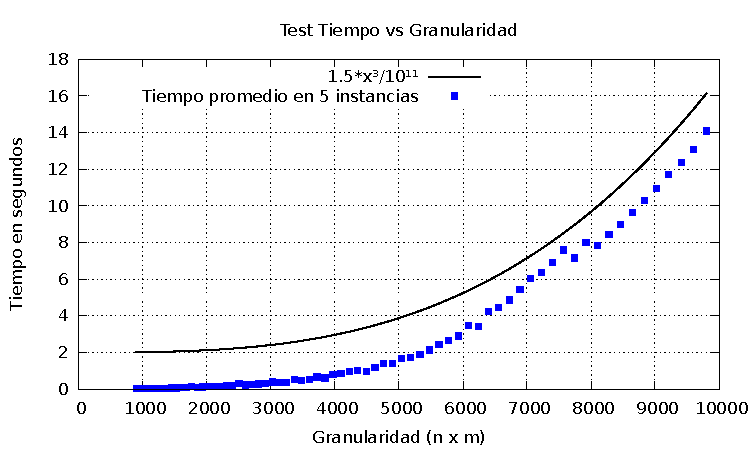
\includegraphics{graphs/granuVstiempo2.pdf}
\caption{Comparación del tiempo de ejecución de diferentes granularidades comparando con una función cúbica.}
\label{gaussVsLU1}
\end{figure}

